%\documentclass[spanish,12pt,a4paper,titlepage,twoside,openright]{scrbook}
\documentclass[12pt,a4paper,titlepage]{report}
%\usepackage[latin1]{inputenc}
\usepackage[utf8]{inputenc}
\usepackage{graphicx}
\usepackage{subfig}
\usepackage{float}
\usepackage{wrapfig}
\usepackage{multirow}
\usepackage{caption}
\usepackage[spanish]{babel}
\usepackage[dvips]{hyperref}
\usepackage{amssymb}
\usepackage{listings}
\usepackage{epsfig}
\usepackage{amsmath}
\usepackage{array}
\usepackage[table]{xcolor}
\usepackage{multirow}
\usepackage{hhline}
\usepackage{cancel}

\usepackage[Sonny]{fncychap}
%\usepackage[Glenn]{fncychap}
%\usepackage[Conny]{fncychap}
%\usepackage[Rejne]{fncychap}
%\usepackage[Bjarne]{fncychap}

\usepackage{subfiles}
\usepackage{framed}
\usepackage{appendix}
\setlength{\topmargin}{-1.5cm}
\setlength{\textheight}{25cm}
\setlength{\oddsidemargin}{0.3cm} 
\setlength{\textwidth}{15cm}
\setlength{\columnsep}{0cm}
%\setkomafont{disposition}{\normalfont\bfseries}
\captionsetup{tablename=Tabla}

\ChNameVar{\bfseries\LARGE\sf}\ChNumVar{\fontsize{62}{65}\selectfont}
\ChTitleVar{\bfseries\LARGE\sf} \ChRuleWidth{2pt} \ChNameAsIs
\ChTitleAsIs
\renewcommand\FmN[4]{}
\newcommand{\HRule}{\rule{\linewidth}{0.5mm}}

\begin{document}


\begin{titlepage}
\begin{center}
\vfill
%\vspace{50cm}
\textsc{\LARGE Facultad de Ingenier\'ia de la Universidad de la Rep\'ublica}\\[1.5cm]
\vspace{2cm}
\textsc{\LARGE Procesamiento Digital de Señales de Audio\\[1cm]Curso 2012}\\[0.5cm]
\vspace{2.3cm}
% Title
\HRule \\[0.4cm]
{ \huge \bfseries Reconocimiento de Tempo}\\[0.4cm]
\HRule \\[1.5cm]
\vspace{2cm}
% Author and supervisor
%\begin{center}
\begin{minipage}{0.4\textwidth}
\begin{flushleft} \large
\emph{Autores:}\\
%\begin{center}
%\begin{LARGE}
Gonzalo \textsc{Gutiérrez}\\ Mat\'ias \textsc{Tailani\'an}
%\end{LARGE}
%\end{center}
\end{flushleft}
\end{minipage}
%\end{center}
\begin{minipage}{0.4\textwidth}
\begin{flushright} \large
\end{flushright}
\end{minipage}

\vspace{2cm}

\vfill
\begin{figure} [h!]
\centering
\subfloat{
\includegraphics[width=0.25\textwidth]{./pics/logoIIE_transparente.png}}\hspace{1cm}
\subfloat{
\includegraphics[width=0.15\textwidth]{./pics/logo_fing_transparente.png}}\hspace{1cm}
\subfloat{
\includegraphics[width=0.15\textwidth]{./pics/logo_udelar.png}}
\end{figure}

% Bottom of the page
{\large \today}
\end{center}
\end{titlepage}

\chapter*{Segunda etapa}

De estudios psicoacústicos sobre la percepción del \emph{beat} se deduce que hay ciertas manipulaciones y simplificaciones que se pueden realizar sobre las señales sin alterar la percepción del \emph{beat}.\\

Consideremos el siguiente experimento: se divide en bandas de frecuencia y se detecta la envolvente de cada banda. Por otro lado se genera un ruido gaussiano y se lo multiplica por la envolvente anterior en cada banda de frecuencia. Se suman las señales de las distintas bandas y se obtiene así un ruido de amplitud modulada. Lo interesante de este experimento es que todavía es posible identificar las características métricas de la señal original. Otros experimentos como tomar solamente la salida de uno de los filtros del banco o combinar linealmente las envolventes de las subbandas, indican que no se pueden realizar dichas simplificaciones, ya que alteran el contenido métrico de la señal.

\section*{Técnicas clásicos}

Para la detección del \emph{beat} comúnmente se utilizan técnicas basadas en una detección estadística, simplemente utilizando la energía de la señal o analizando la energía en una banda de frecuencias seleccionada, o técnicas de filtrado y detección del ritmo mediante bancos de filtros y procesamiento de frecuencias seleccionadas.\\

Una de las técnicas más utilizadas, por casi todos los algoritmos de detección y tracking del \emph{beat}, es la división en subbandas de frecuencias. A modo de ejemplo se muestra un banco de 6 filtros que puede ser utilizado: el primero es un pasabajos de frecuencia de corte en 200Hz, el siguiente un pasabanda entre 200Hz y 400Hz, otro entre 400Hz y 800Hz, otro de 800Hz a 1600Hz, de 1600Hz a 3200Hz, y por último un pasaaltos de frecuencia 3200Hz. Una vez pasada la señal por el banco de filtros se realiza la detección de envolvente en cada subbanda.\\

Luego de extraída la envolvente y procesada con alguna técnica en cada canal, una técnica clásica para determinar el \emph{tempo} de la señal es utilizar un banco de filtros resonadores.
Considerando un filtro de retardo T y ganancia $\alpha$, si la señal de entrada tiene amplitud A y periodo K, la señal de salida va a presentar valores altos si T=K (o eventualmente algún divisor). De lo contrario se obtiene una salida chica. Al final del algoritmo se obtiene una especie de puntaje para cada filtro resonador. El filtro que obtenga más puntaje será el que tenga un retardo más parecido al período de la señál.\\

El ritmo como concepto musical es intuitivamente fácil de entender pero de alguna manera difícil de definir. La experiencia del ritmo involucra movimiento, regularidad, agrupamiento, acentuación y diferenciación (Handel, 1989, p. 384). No hay un ``ground truth'' que se pueda encontrar en simples medidas de la señal. El único \emph{ground truth} es el acuerdo que se realiza entre las percepciones de distintas personas que escuchan la pieza musical. Pensando en técnicas de tracking de \emph{beat} automáticas, más allá de todas las técnicas utilizadas, es necesario dar en algún momento, un salto semántico que nos permita obtener un resultado similar a nuestro \emph{ground truth}: la percepción humana. Para lograr este objetivo se pueden realizar algunas consideraciones heurísticas como acotar el rango de tempo que una persona tiene a marcar al escuchar una pieza. Una regla simple es por ejemplo poner un umbral donde todas las piezas que tengan un tempo detectado superior, se utilice la mitad del tempo detectado.

\subsection*{Musical Beat Tracking via Kalman Filtering and Noisy Measurements Selection}

En la etapa de preprocesado se realiza la detección del comienzo (\emph{Onset Detection}) y estimación del período (\emph{Periodicity Estimation}).\\

El \emph{onset} de una señal proporciona el cambio de intensidad de la pieza musical a lo largo del tiempo. Básicamente se distinguen 2 tipos de cambios que producen la aparición de un \emph{onset}:
\begin{itemize}
	\item pulsos causados por la percusión, que se reflejan como pulsos ruidosos de elevada energía
	\item cambios de pitch y armonías debido a la llegada de una nueva nota
\end{itemize}

\begin{figure}[h!]
	\vspace{-20pt}
	\begin{center}
	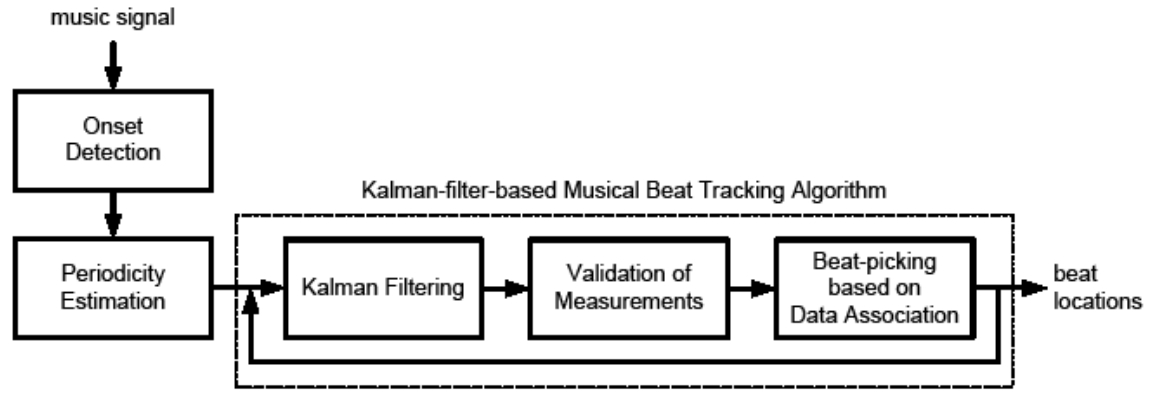
\includegraphics[width=0.65\textwidth]{./pics/kalman_blocks.jpg}
	\end{center}
	\caption{Diagrama de bloques}
	\label{fig:kalman_blocks}
\end{figure}

Se utiliza el método de la distancia cepstral para identificar los inicios musicales\footnote{L. Rabiner, ``A tutorial on hidden Markov models and selected applications
inspeech recognitio'', Proceedings of the IEEE, vol. 77, No. 2, pp. 257-286, 1989.} y la función de autocorrelación para determinar el período.\\

Para el filtrado de Kalman se modela al sistema de Beat Tracking como un sistema dinámico de ecuaciones lineales donde el Tempo musical puede ser modelado como una variable de estado de un sistema dinámico estocástico. Aquí, se utiliza el modelo dinámico propuesto por Cemgil\footnote{ A. T. Cemgil, B. Kappen, P. Desain, and H. Honing, ``On tempo
tracking: tempogram representation and Kalman filtering,'' J. New Music
Res., vol. 28, pp. 259-273, 2001.} para formular el problema del Beat Tracking  en un marco probabilístico.

\subsubsection*{Selección de los Beats}
El rendimiento del Beat Tracking basado sólo en el filtrado de Kalman no alcanza una muy buena performance. Para mejorar su rendimiento, necesitamos una forma más inteligente para localizar beats reales a partir de la señal de audio. Se aplicará entonces una técnica de asociación probabilística de datos (\textbf{PDA}), o la mejorada, \textbf{Enhanced PDA (EPDA)}.

\subsection*{Improved Perceptual Tempo Detection of Music}

Un esquema general muy ilustrativo del algoritmo propuesto se puede ver en la figura \ref{fig:esquema}.\\

\begin{figure}[h!]
	\vspace{-20pt}
	\begin{center}
	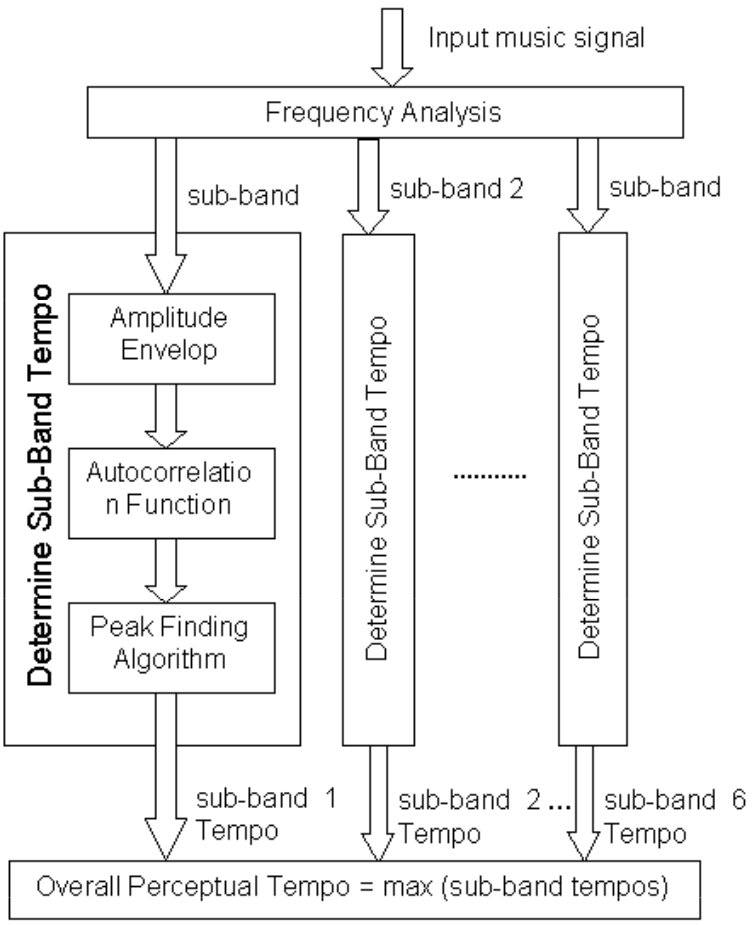
\includegraphics[width=0.4\textwidth]{./pics/esquema.jpg}
	\end{center}
	\caption{Esquema}
	\label{fig:esquema}
\end{figure}

\begin{enumerate}
\item \textbf{Frequency Analysis}: Se divide la señal a analizar en seis bandas diferentes (0-200Hz, 200-400Hz, 400-800Hz, 800-1600Hz, 1600-3200Hz y más de 3200Hz)
\item \textbf{Autocorrelation function}: La periodicidad de las señales de cada sub-banda se detecta utilizando la función de autocorrelación (ACF).
\item \textbf{Peak Finding Algorithm}: Se aplica el algoritmo para encontrar el \emph{tempo} de cada sub-banda. El algoritmo estima el \emph{tempo} mediante la búsqueda del mayor pico con tiempo de retardo mayor a cero. Sin embargo, este pico por lo general no suele reflejar el \emph{tempo perceptual}. El algoritmo de búsqueda de pico propuesto debe determinar el \emph{tempo} en cada sub-banda mediante la búsqueda del pico con el retardo de tiempo más corto mayor a cero, por encima del 20\% de la energía total. El umbral de 20\% se determinó empíricamente.\\
tempo perceptual de la señal musical está determinada por la búsqueda del mayor \emph{tempo} entre los \emph{tempos} de cada sub-banda.
\end{enumerate}

\subsubsection*{IPTE: descripción del algoritmo PTE mejorado}

\begin{enumerate}
\item Se divide a la pieza en segmentos de longitudes fijas (por ejemplo de 10 segundos)
\item Se aplica el algoritmo de PTE para cada segmento para obtener el tempo de ese segmento.
\item Se encuentra el tempo ocurrido con mayor frecuencia entre los tempos del segmento, según la determinación de la similitud en peso en cada segmento.
\item Determinar la probabilidad del peso para cada segmento de tempo para que sea más probable que el tempo del segmento anterior sea seleccionado como tempo perceptual global.
\item Determinar el tempo general perceptual de la pieza musical a partir de la información obtenida en los pasos 2, 3 y 4.
\end{enumerate}


\subsection*{Beat Tracking based on Multiple-agent Architecture}

La arquitectura de múltiples agentes se basa en que estos agentes llevan diferentes estrategias en paralelo e interactúan y compiten entre sí para seguir a los \emph{beats}.\\

\begin{wrapfigure}{l}{0.45\textwidth}
	\vspace{-10pt}
	\begin{center}
	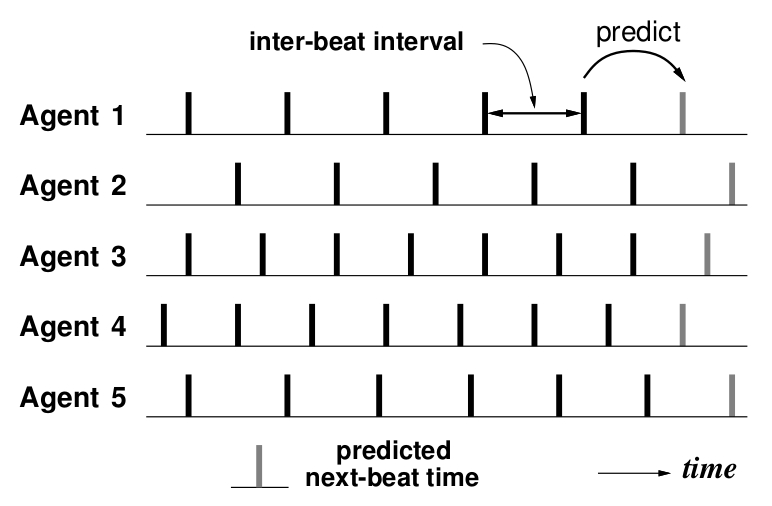
\includegraphics[width=.4\textwidth]{./pics/agents.jpg}
	\end{center}
	\vspace{-10pt}
	\caption{Agentes}
	\label{fig:agents}
	\vspace{-40pt}
\end{wrapfigure}

Los agentes deben cumplir que:
\begin{enumerate}
\item El agente interactúa con otros agentes para llevar a cabo una determinada tarea
\item El agente evalúa su propio comportamiento
\item El agente se adapta a la entrada mediante el ajuste de su propio comportamiento
\end{enumerate}

Cada agente mantiene una hipótesis de posición de beat, que consiste en una predicción del tiempo de \emph{beat} siguiente.\\

\begin{wrapfigure}{r}{0.45\textwidth}
	\vspace{-20pt}
	\begin{center}
	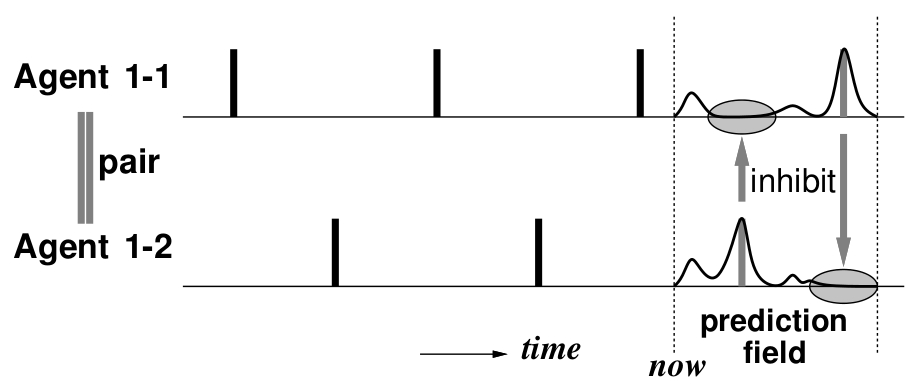
\includegraphics[width=.4\textwidth]{./pics/agent_pair.jpg}
	\end{center}
	\vspace{-10pt}
	\caption{Par de agentes}
	\label{fig:agent_pair}
	\vspace{-10pt}
\end{wrapfigure}

Todos los agentes se agrupan en pares que tienen diferentes estrategias para el Beat Tracking. Cada agente en el par examina el mismo inter-beat interval usando los mismos resultados de análisis de frecuencia. Para predecir los tiempos de compás próximos cooperativamente, un agente interactúa con el otro agente en el mismo par a través de una predicción de campo. La predicción de campo es una curva de esperanza que representa cuando el ritmo próximo se espera que ocurra.

\subsubsection*{Descripción del sistema}
Las dos etapas principales del proceso son el \textbf{Análisis de Frecuencia}, en la que varias señales utilizadas por los agentes se detectan y la \textbf{Predicción de Beat}, en el que múltiples hipótesis de las posiciones de beat son examinados por varios agentes.\\

\begin{wrapfigure}{l}{0.6\textwidth}
	\vspace{-20pt}
	\begin{center}
	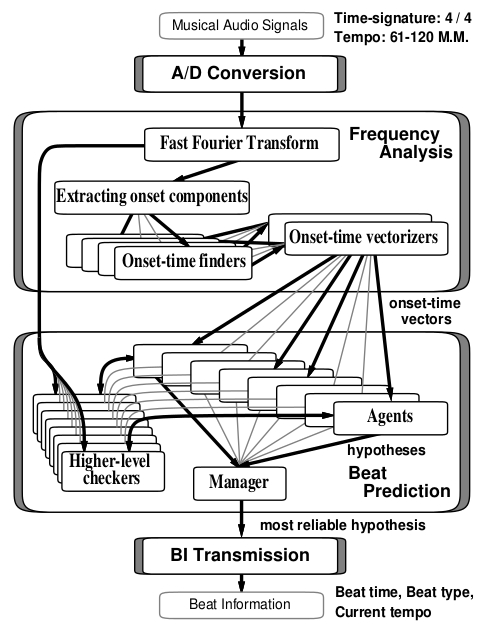
\includegraphics[width=.5\textwidth]{./pics/agents_blocks.jpg}
	\end{center}
	\vspace{-10pt}
	\caption{Diagrama de bloques}
	\label{fig:agents_blocks}
\end{wrapfigure}

En la etapa de Análisis de Frecuencia, el sistema usa múltiples buscadores de onsets, detectándolos en varios rangos de frecuencia diferentes. Estos resultados se transforman en una representación vectorial (llamado onset-time vectors).\\

En la etapa de predicción del \emph{be}at, el sistema gestiona múltiples agentes que, de acuerdo con diferentes estrategias, hacen hipótesis en paralelo basados en estos vectores tiempo de \emph{onsets}. Cada agente, primero calcula el \emph{inter-beat interval} y predice el siguiente  tiempo de \emph{beat}, de donde luego se deduce el tipo de compás mediante la comunicación con un corrector de nivel superior, y evalúa la confiabilidad de su propia hipótesis. El gestor reúne todas las hipótesis y luego determina la salida final sobre la base de la más fiable.

\end{document}